\chapter{Vorlesung}
\subsection{Lemma}
Für jeden Knoten $x$ in einem Fibonacci-Heap gilt, dass die Zahl aller Knoten im Unterbaum von $x$ mindestens $\Phi^k$ beträgt, wobei $k = \grad(x)$.
\subsection{Beweis}
\begin{wrapfigure}{L}{0.5\linewidth}
	\centering
	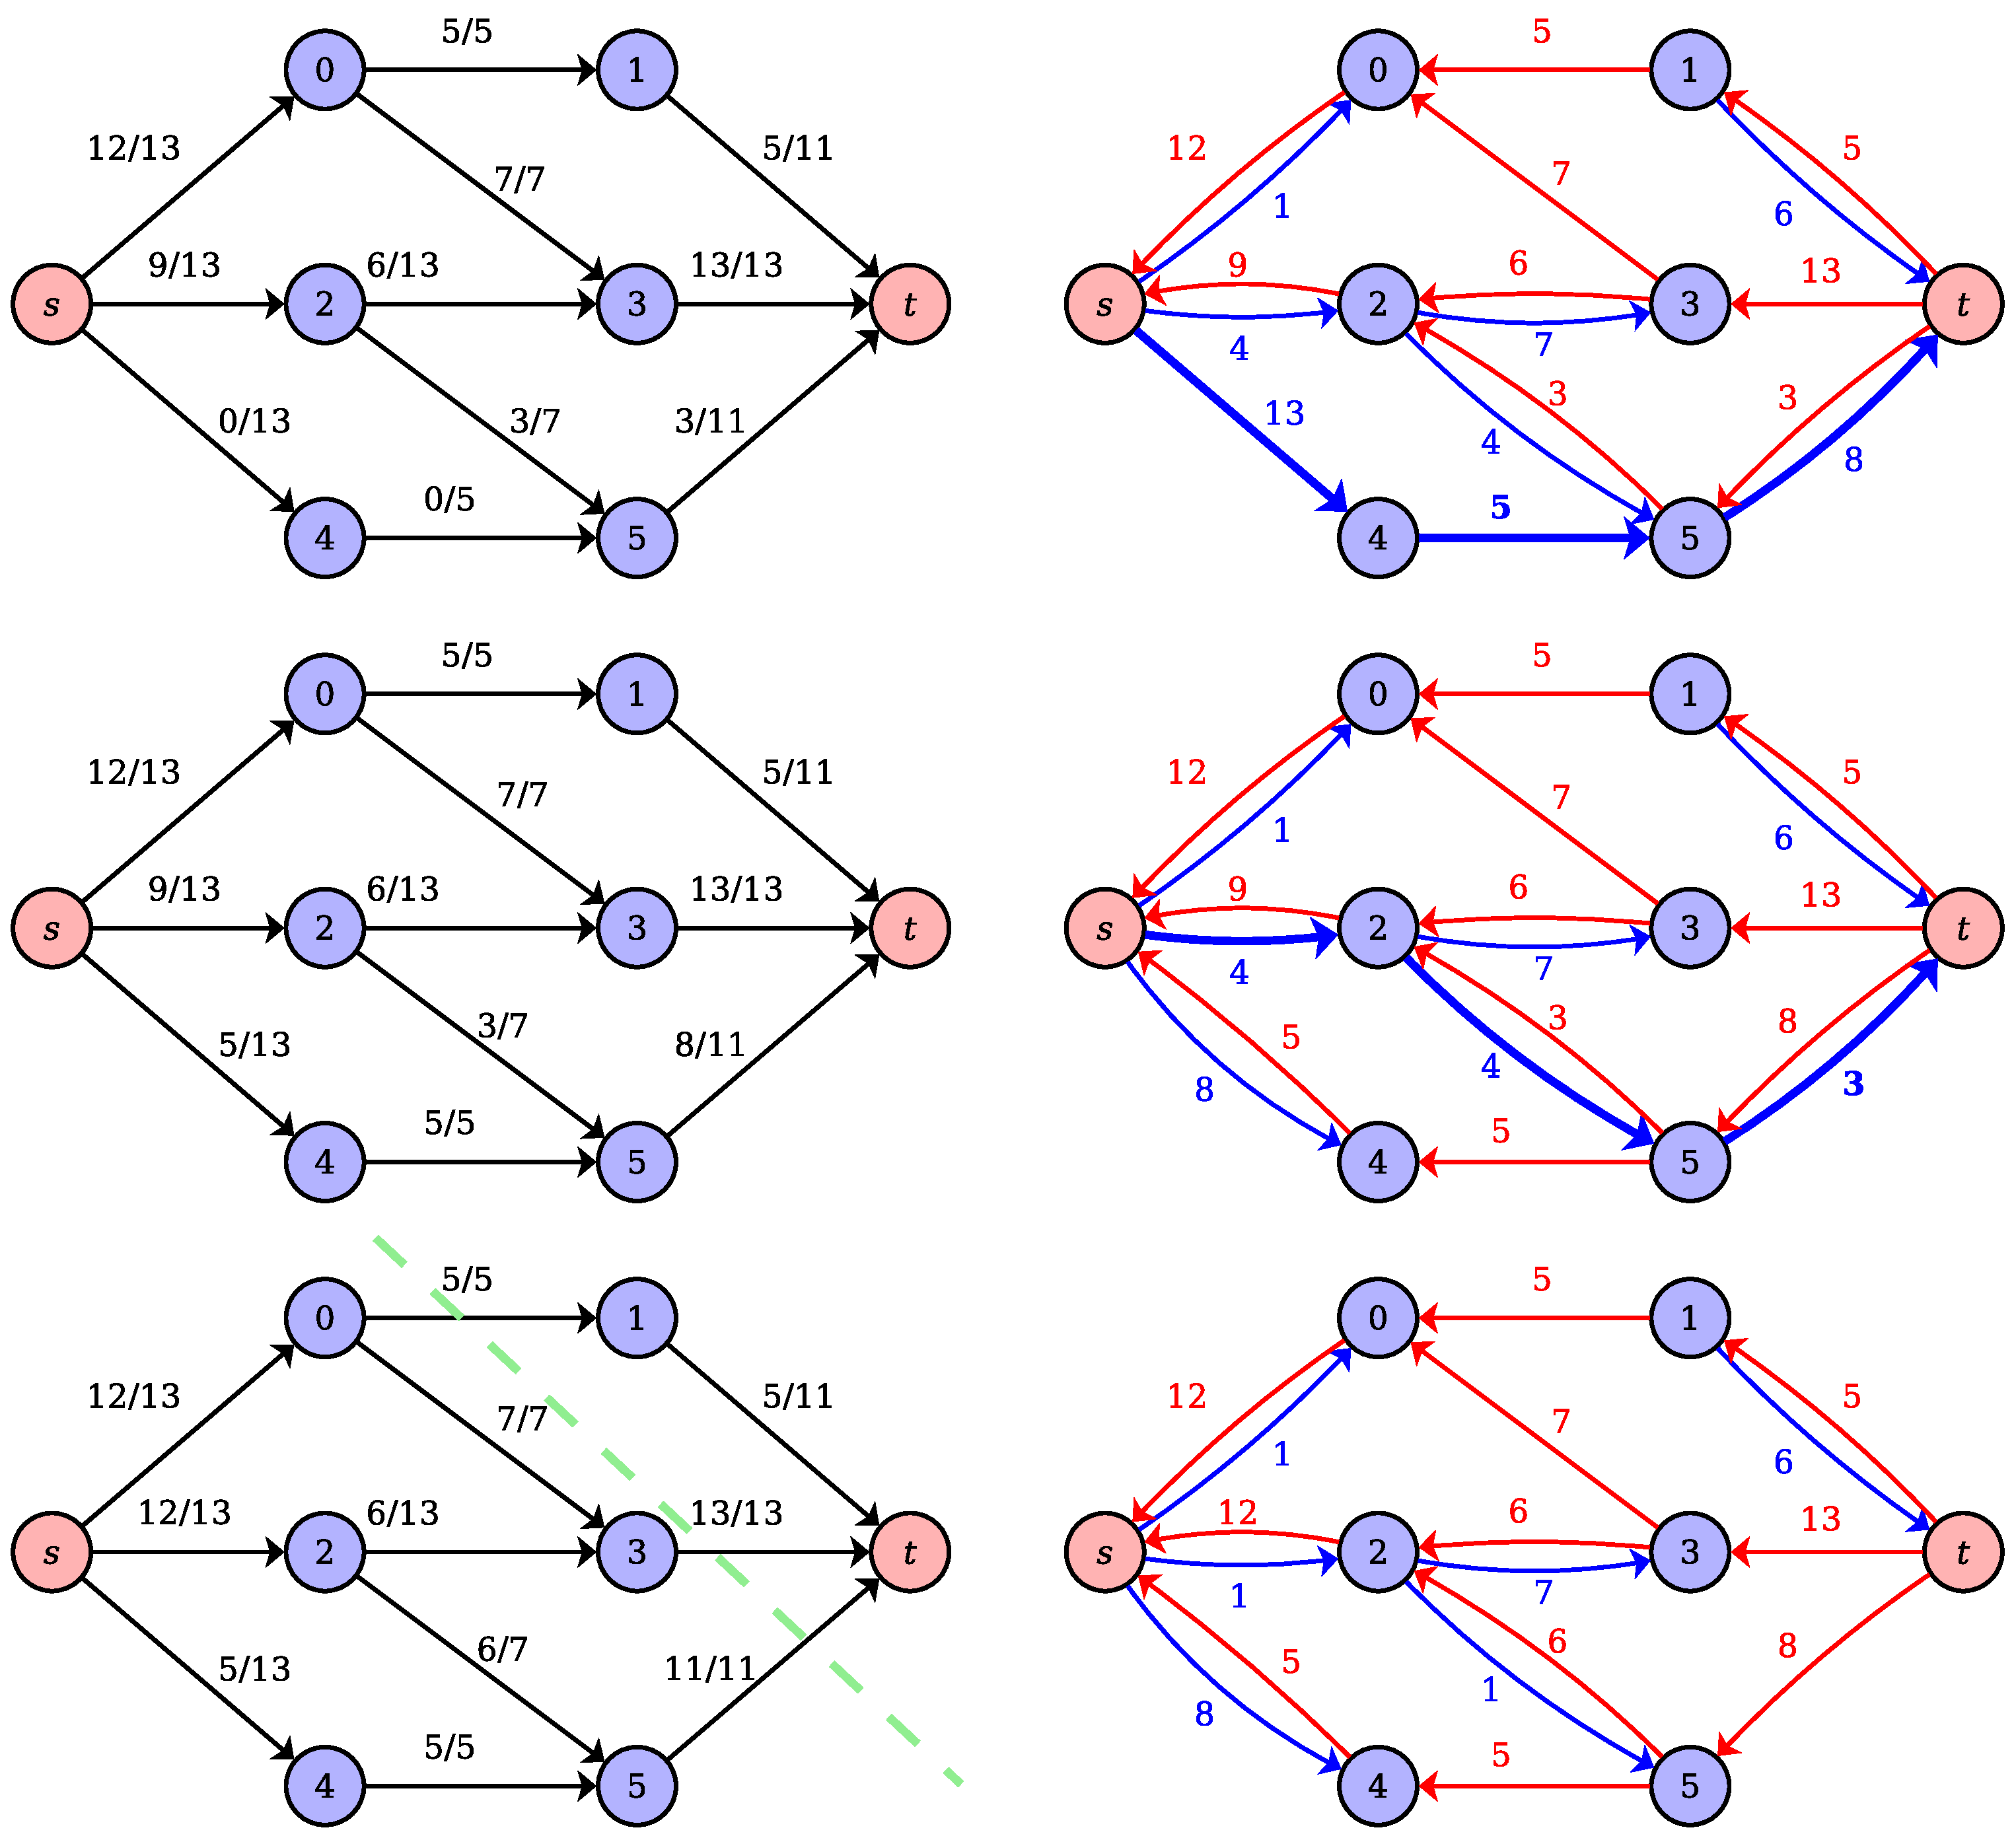
\includegraphics[width=\linewidth]{22/Grafik/Diagramm1}
	\caption{Schaubild zum Beweis}
	\label{fig:beweis}
\end{wrapfigure}
Seien $y_1, y_2,\ldots,y_k$ die aktuellen Kindknoten von $x$, nummeriert in der Reihenfolge, wie sie (letztmalig) Kindknoten von $x$ geworden sind. Zum Zeitpunk, zu dem $y_i$ Kindknoten von $x$ geworden ist, existieren bereits die $i-1$ Kindknoten $y_1, y_2,\ldots,y_{i-1}$. $\Rightarrow\grad(x)\geq i-1$\\ 
$y_i$ kann nur Kind von $x$ werden, wenn $x$ und $y_i$ gleichen Grad haben. $\Rightarrow\grad(y_i)\geq i-1$\\
Da $y_i$ im Folgenden höchstens einen Kindknoten verlieren kann, gilt:
\[ \grad(y_i) \geq i-2 \]
Sei $S_k$ die Mindestanzahl von Knoten in einem Unterbaum eines Knoten $x$ vom Grad $k$
\[ S_k \geq 1+1+\sum_{i=2}^{k} S_{i-2} \]
Wir zeigen
\[ S_k\overset{(2)}{\geq} f_{k+2}\footnote{$k-2$-te Fibonacci Zahl}\overset{(1)}{\geq}\Phi^k \]

\begin{wraptable}[-5]{R}{0.3\linewidth}
	\centering
	\begin{tabular}{ccccccc}
		$f_0$&$f_1$&$f_2$&$f_3$&$f_4$&$f_5$&$\ldots$\\
		$0$&$1$&$1$&$2$&$3$&$5$& 
	\end{tabular}
\end{wraptable}
\paragraph{(1)}
\[ f_{k+2}\geq \Phi^k \]
\[ k=0~:~ f_2=1\geq\Phi^0=1 \]
\[ k=1~:~ f_3=2\geq\Phi^1=1,6181\ldots \]
\[ f_{k+2} = f_{k+1}+f_k \geq \Phi^{k-1}+\Phi{k-2}=\footnote{$\Phi^2=\Phi+1$} \Phi{k-2}(\Phi+1)=\Phi{k-2}\cdots\Phi^2=\Phi^k \]
\paragraph{(2)}
\[ S_k \geq f_{k+2} \text{?}\]
\[ S_k\geq 2+\sum_{i=2}^{k}S_{i-2} \]
\[ k=0~:~S_0\geq f_2=1~~\checkmark \]
\[ k=1~:~S_1\geq f_3=2~~\checkmark \]
\[ S_k \geq 2+\sum_{i=2}^{k}f_i\text{, da wegen Induktions-Annahme }S_{i-2}\geq f_{(i-2+2)}=f_i \text{ für }i<k \]
\paragraph{Zu zeigen}
\[ 2 + \sum_{i=2}^{k}f_i \geq f_{k+2} \]
\paragraph{Es gilt:}
\[ 1+\sum_{i=1}^{k}f_i=f_{k+2} \]
\[ k=0~:~1=f_2~\checkmark \]
\[ k=1~:~1+f_1=f_3=2~\checkmark \]
\[ 1+\sum_{i=1}^{k+1} = (1+\sum_{i=1}^{k}f_i)+f_{k+1} = f_{k+2}+f_{k+1}=f_{k+3} \]
\begin{flushright}
	q.e.d.
\end{flushright}
Aus dem Lemma folgt, dass in einem Fibonacci-Heap für $n$\footnote{$\Phi^k\leq n$} Elemente zu keinem Zeitpunkt einen Knoten vom Grad $\log_\phi n = k$ auftauchen kann. Insbesondere ist die Wurzelliste nach einer Konsolidierung auch nur $\log_\Phi n$ lang, weil dort nur Knoten unterschiedlichen Grades auftauchen. 